% =====================================================================================
%  Splaire (Aire medido en cada Metro) — Informe del rol de Modelado y Validación (Estudio de Caso 3)
%  Compilar:  pdflatex informe_modelado_validacion.tex   (dos veces, por las referencias)
%  Overleaf : subir la carpeta docs/informe completa (incluye figuras/ y generado/).
%  Todos los números provienen de generado/valores.tex, producido por
%  `python modelado_validacion.py` (no se transcriben a mano).
% =====================================================================================
\documentclass[conference,a4paper]{IEEEtran}
\usepackage[utf8]{inputenc}
\usepackage[T1]{fontenc}
\usepackage{lmodern}
\usepackage[spanish,es-noshorthands,es-tabla,es-nodecimaldot]{babel}
\usepackage{amsmath,amssymb}
\usepackage{graphicx}
\usepackage{booktabs}
\usepackage{array}
\usepackage{cite}
\usepackage{xcolor}
\usepackage{listings}
\usepackage{url}
\usepackage[hidelinks]{hyperref}

% Generado automáticamente por modelado_validacion.py — no editar a mano.
\newcommand{\RMSEnak}{1.045}
\newcommand{\EMAXnak}{1.528}
\newcommand{\MAEnak}{0.987}
\newcommand{\PEORnak}{E7}
\newcommand{\RMSEnat}{1.529}
\newcommand{\EMAXnat}{2.621}
\newcommand{\RMSEsuj}{1.852}
\newcommand{\RMSElin}{3.787}
\newcommand{\RMSElag}{8.483}
\newcommand{\EMAXlag}{16.333}
\newcommand{\RMSEher}{2.080}
\newcommand{\RMSEpch}{2.366}
\newcommand{\REDlin}{72.4}
\newcommand{\REDlag}{87.7}
\newcommand{\REDnat}{31.7}
\newcommand{\LEBlag}{17.85}
\newcommand{\LEBlagkm}{0.32}
\newcommand{\LEBnak}{1.97}
\newcommand{\LEBnat}{1.54}
\newcommand{\LEBlagTreinta}{3.4\times10^{6}}
\newcommand{\LEBnakTreinta}{1.97}
\newcommand{\RAZONnodal}{49}
\newcommand{\LOCuno}{0.137}
\newcommand{\LOCdos}{0.037}
\newcommand{\LOCtres}{0.012}
\newcommand{\LOCnakBorde}{0.044}
\newcommand{\LOClagBorde}{4.03}
\newcommand{\EXTlag}{4}
\newcommand{\VTlag}{4.28}
\newcommand{\VTnak}{0.08}
\newcommand{\MINnak}{41.98}
\newcommand{\ORDnak}{3.99}
\newcommand{\ORDnat}{2.00}
\newcommand{\ORDsujex}{4.01}
\newcommand{\ORDsuj}{2.02}
\newcommand{\ORDlin}{2.00}
\newcommand{\VERmax}{1.4\times10^{-14}}
\newcommand{\CONTmax}{1.4\times10^{-14}}
\newcommand{\CONDnat}{2.77}
\newcommand{\CONDnak}{2.82}
\newcommand{\FACnakBorde}{2.48}
\newcommand{\FACnatBorde}{1.50}
\newcommand{\FAClagBorde}{24.5}
\newcommand{\FAClin}{1.225}
\newcommand{\FACnakRMS}{1.80}
\newcommand{\FACnatRMS}{1.50}
\newcommand{\MCnak}{4.17}
\newcommand{\MCnat}{3.78}
\newcommand{\MClin}{4.78}
\newcommand{\MClag}{26.0}
\newcommand{\MCher}{3.83}
\newcommand{\MCganaNak}{31}
\newcommand{\PCTnak}{1.7}
\newcommand{\SIGef}{0.58}
\newcommand{\NMC}{2000}
\newcommand{\SEMILLA}{2024}
\newcommand{\AMdesde}{2.11}
\newcommand{\AMhasta}{6.59}
\newcommand{\ROdesde}{3.49}
\newcommand{\ROhasta}{4.68}
\newcommand{\DESFASEsplines}{5}
\newcommand{\DESFASElin}{226}
\newcommand{\RUNGElagIni}{0.44}
\newcommand{\RUNGElagFin}{59.8}
\newcommand{\RUNGEsplFin}{0.0032}
\newcommand{\RUNGEnodosFin}{21}
\newcommand{\SPPnakIni}{15.7}
\newcommand{\SPPnakFin}{16.1}
\newcommand{\SPPsujIni}{-7.6}
\newcommand{\SPPsujFin}{-7.7}
\newcommand{\BANDAmax}{11.23}
\newcommand{\BANDAmaxkm}{8.4}
\newcommand{\BANDAmin}{6.93}
\newcommand{\BANDAminkm}{4.4}
\newcommand{\BANDAborde}{9.69}
\newcommand{\BANDAinterior}{8.96}
\newcommand{\DESFASEherPch}{45}
\newcommand{\ROlinDesde}{3.71}
\newcommand{\ROlinHasta}{4.50}
\newcommand{\DIFbordeNat}{0.79}
\newcommand{\DIFintNat}{0.21}


\newcommand{\ugm}{\ensuremath{\mu}g/m\textsuperscript{3}}
\newcommand{\PMdc}{PM\textsubscript{2.5}}
\newcommand{\nak}{\emph{not-a-knot}}
\renewcommand{\IEEEkeywordsname}{Palabras clave}
\renewcommand{\lstlistingname}{Código}
\setcounter{dbltopnumber}{2}
\renewcommand{\dbltopfraction}{0.85}
\renewcommand{\dblfloatpagefraction}{0.8}
\renewcommand{\bottomfraction}{0.55}
\raggedbottom

\definecolor{codigo}{HTML}{F5F7FA}
\definecolor{comentario}{HTML}{2563EB}
\lstset{language=Python, basicstyle=\ttfamily\scriptsize, backgroundcolor=\color{codigo},
  commentstyle=\color{comentario}\itshape, keywordstyle=\bfseries, frame=none, columns=fullflexible,
  keepspaces=true, showstringspaces=false, xleftmargin=2pt, aboveskip=4pt, belowskip=2pt,
  literate={á}{{\'a}}1 {é}{{\'e}}1 {í}{{\'i}}1 {ó}{{\'o}}1 {ú}{{\'u}}1 {ñ}{{\~n}}1 {ŷ}{{\^y}}1}

\begin{document}

\title{Splaire: \emph{Aire medido en cada Metro}\\[2pt]
{\Large Modelado y validación de splines cúbicos para sensores virtuales de \PMdc}}

\author{\IEEEauthorblockN{Estudiantes:\\
Juan David Garrido (Ingeniero de Algoritmos y Simulación)\\
Edwin Quiñones (Ingeniero de Integración y Estrategia)\\
Miguel Angel Laiton (Ingeniero de Modelado y Validación)}
\IEEEauthorblockA{Equipo Splaire · Análisis Numérico para Ingeniería · Estudio de Caso 3 (\emph{Air Health Analytics})\\
Repositorio: \url{https://github.com/JuanDGarridoR/Proyecto---Analisis-Numerico}}}

\maketitle

\begin{abstract}
Se formula el problema de estimar la concentración de \PMdc{} cada 0.1\,km a partir de 10 estaciones
equidistantes en un corredor de 9\,km, se justifica la condición de frontera del spline cúbico y se valida
el modelo. La frontera \nak{} se elige con evidencia: en la validación cruzada \emph{leave-one-out} (LOOCV)
sobre los 8 nodos internos obtiene RMSE\,=\,\RMSEnak{}\,\ugm{} y error máximo \EMAXnak{}\,\ugm{}
(\PEORnak), un \REDlin\,\% menos RMSE que la interpolación lineal y un \REDlag\,\% menos que Lagrange.
Se cuantifica el fenómeno de Runge en los nodos del corredor (constante de Lebesgue \LEBlag{} para Lagrange
frente a \LEBnak{} para el spline) y se verifica el orden de convergencia $O(h^4)$ (observado \ORDnak).
Finalmente, se analiza la robustez frente a ruido instrumental $\sigma=2.5$\,\ugm: el ruido se amplifica
$\times$\FACnakBorde{} en las estaciones de borde, pero los tramos de alerta son insensibles a la frontera
elegida (desfase $\le$\,\DESFASEsplines\,m).
\end{abstract}

\begin{IEEEkeywords}
spline cúbico, fenómeno de Runge, constante de Lebesgue, validación cruzada, condiciones de frontera, \PMdc.
\end{IEEEkeywords}

% -------------------------------------------------------------------------------------
\section{Introducción}
Splaire ---\emph{Aire medido en cada Metro}--- genera \emph{sensores virtuales} de \PMdc{}: a partir de 10 estaciones fijas (una por
kilómetro) interpola la concentración en una malla de 91 puntos ($\Delta x=0.1$\,km) para emitir
alertas sanitarias (amarilla $\ge 70$\,\ugm, roja $\ge 90$\,\ugm). Este informe documenta el trabajo del
rol de Modelado y Validación, que corresponde a las secciones §2, §3 y §5 del cuaderno
\texttt{AirSpline\_Caso3.ipynb} y al módulo \texttt{modelado\_validacion.py} del repositorio. Se distinguen
dos preguntas: \emph{verificación} (¿se resuelven bien las ecuaciones?) y \emph{validación} (¿el modelo
predice bien las estaciones que no ve?). Además de la LOOCV exigida, se analiza la robustez de la propia
validación frente al ruido de los sensores.

% -------------------------------------------------------------------------------------
\section{Formulación del problema}\label{sec:formulacion}
\begin{figure*}[!t]
\centering
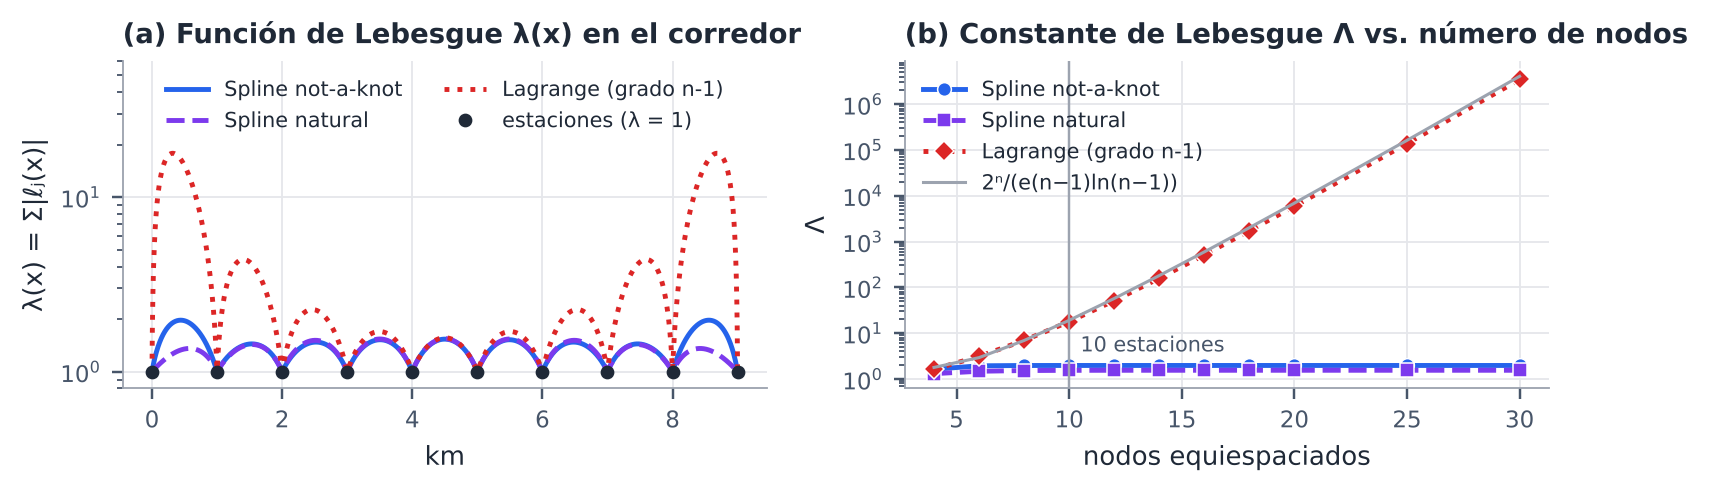
\includegraphics[width=0.92\textwidth]{figuras/fig2_runge_lebesgue.png}
\caption{Fenómeno de Runge cuantificado. (a) Función de Lebesgue en los nodos del corredor: Lagrange
amplifica hasta $\times$\LEBlag{} cerca de los extremos; el spline se mantiene por debajo de 2.
(b) Crecimiento exponencial de $\Lambda$ para Lagrange (sigue la asintótica) y acotado para el spline.}
\label{fig:runge}
\end{figure*}
\begin{table*}[!t]
\caption{Condiciones de frontera evaluadas (orden observado al refinar $h$ y RMSE de la LOOCV, en \ugm)}
\label{tab:fronteras}
\centering\footnotesize
\setlength{\tabcolsep}{4pt}
\begin{tabular}{@{}>{\raggedright}p{1.7cm} >{\raggedright}p{3.4cm} >{\raggedright}p{9.6cm} c c@{}}
\toprule
Frontera & Condición & Hipótesis y comentario para el corredor & Orden & RMSE \tabularnewline
\midrule
Natural & $S''(0)=S''(9)=0$ & Supone curvatura nula en los extremos, pero los datos indican $S''_{\text{nak}}(0)=\SPPnakIni$ y
$S''_{\text{nak}}(9)=\SPPnakFin$: hipótesis falsa, error $O(h^2)$ en los bordes. & \ORDnat & \RMSEnat \tabularnewline
Sujeta & $S'(0)=f'_0$, $S'(9)=f'_9$ & Las pendientes no se miden; con \texttt{np.gradient} (unilateral, $O(h)$) el orden cae a
\ORDsuj{} y la curvatura de borde cambia de signo ($S''(0)=\SPPsujIni$). Con $f'$ exacta: \ORDsujex. & \ORDsuj & \RMSEsuj \tabularnewline
\textbf{Not-a-knot} & $S'''$ continua en $x_1$, $x_8$ & Sin hipótesis física: la curvatura de borde la determinan los datos. & \textbf{\ORDnak} & \textbf{\RMSEnak} \tabularnewline
Periódica & $S,S',S''$ iguales en 0 y 9 & Exige $y_0=y_9$ y un dominio cerrado; el corredor es abierto y $45\neq42$. Descartada. & --- & --- \tabularnewline
\midrule
Lineal & --- & Sólo $C^0$; recorta los picos. & \ORDlin & \RMSElin \tabularnewline
Lagrange & grado 9 & Inestable con nodos equidistantes (Sec.~\ref{sec:runge}). & --- & \RMSElag \tabularnewline
\bottomrule
\end{tabular}
\end{table*}
\subsection{Datos y modelo}
Los nodos son $x_i=i$\,km, $i=0,\dots,9$ ($n=9$ tramos, $h=1$\,km), con lecturas
\[ y=(45,\,52,\,68,\,85,\,92,\,88,\,79,\,63,\,48,\,42)\ \text{\ugm}. \]
En cada tramo $[x_i,x_{i+1}]$ el spline es
\begin{equation}
S_i(x)=a_i+b_i(x-x_i)+c_i(x-x_i)^2+d_i(x-x_i)^3 .
\end{equation}
Hay $4n=36$ incógnitas: $2n=18$ condiciones de interpolación, $2(n-1)=16$ de continuidad de $S'$ y
$S''$ en los nodos internos (clase $C^2$) y 2 de frontera. Con $a_i=y_i$ y $c_i=S''(x_i)/2$ el problema se
reduce a un sistema en las $c_i$~\cite{burden2017}:
\begin{equation}
\begin{aligned}
&h_{i-1}c_{i-1}+2(h_{i-1}+h_i)c_i+h_ic_{i+1}\\
&\qquad=\tfrac{3}{h_i}(a_{i+1}-a_i)-\tfrac{3}{h_{i-1}}(a_i-a_{i-1}),
\end{aligned}
\end{equation}
para $i=1,\dots,n-1$, y luego $b_i=\frac{a_{i+1}-a_i}{h_i}-\frac{h_i}{3}(2c_i+c_{i+1})$,
$d_i=\frac{c_{i+1}-c_i}{3h_i}$.

\subsection{Sistema del caso}
Con $h=1$ la ecuación queda $c_{i-1}+4c_i+c_{i+1}=3(y_{i+1}-2y_i+y_{i-1})$. Para la frontera natural
($c_0=c_9=0$):
\begin{equation}\setlength{\arraycolsep}{2.4pt}
\begin{bmatrix}4 & 1 & 0 & 0 & 0 & 0 & 0 & 0 \\ 1 & 4 & 1 & 0 & 0 & 0 & 0 & 0 \\ 0 & 1 & 4 & 1 & 0 & 0 & 0 & 0 \\ 0 & 0 & 1 & 4 & 1 & 0 & 0 & 0 \\ 0 & 0 & 0 & 1 & 4 & 1 & 0 & 0 \\ 0 & 0 & 0 & 0 & 1 & 4 & 1 & 0 \\ 0 & 0 & 0 & 0 & 0 & 1 & 4 & 1 \\ 0 & 0 & 0 & 0 & 0 & 0 & 1 & 4\end{bmatrix}
\begin{bmatrix}c_1\\c_2\\c_3\\c_4\\c_5\\c_6\\c_7\\c_8\end{bmatrix}=
\begin{bmatrix}27 \\ 3 \\ -30 \\ -33 \\ -15 \\ -21 \\ 3 \\ 27\end{bmatrix}
\label{eq:sistema}\end{equation}

La matriz es estrictamente diagonal dominante ($4>1+1$), luego no singular; sus valores propios
$4+2\cos(k\pi/9)\in(2,6)$ dan $\kappa_2=\CONDnat$, y el algoritmo de Thomas la resuelve en $O(n)$ sin
pivoteo. Para \nak{} ($d_0=d_1$, $d_7=d_8$) se elimina $c_0=2c_1-c_2$ (y su simétrico $c_9$): la primera y
la última fila pasan a $6c_1=r_1$ y $6c_8=r_8$, con $\kappa_2=\CONDnak$. Para mallas no uniformes (las que
aparecen en la LOOCV) se usa la forma general de la eliminación, implementada en el módulo.

% -------------------------------------------------------------------------------------
\section{Selección de la condición de frontera}
La Tabla~\ref{tab:fronteras} resume la evaluación. El criterio es doble: que la hipótesis tenga sentido
físico y que el error de validación sea mínimo.

La elección \nak{} coincide con la del cuaderno (\texttt{BC\_PRINCIPAL}) y reduce el RMSE un
\REDnat\,\% frente a la natural. La diferencia entre ambas se concentra en los tramos de borde
($\max|\Delta S|=\DIFbordeNat$\,\ugm{} en km 0--1 y 8--9 frente a \DIFintNat\,\ugm{} en el interior).

% -------------------------------------------------------------------------------------
\section{Por qué el spline evita el fenómeno de Runge}\label{sec:runge}
\subsection{Error y estabilidad del polinomio de grado alto}
\begin{figure*}[!t]
\centering
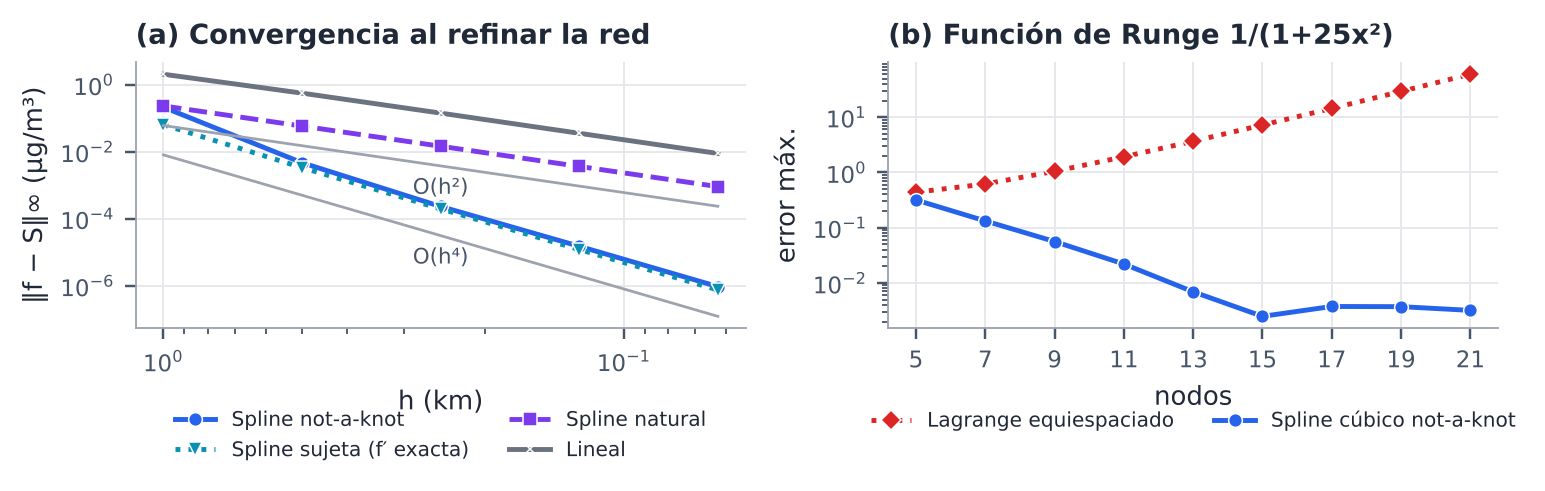
\includegraphics[width=0.92\textwidth]{figuras/fig3_convergencia.png}
\caption{Verificación del orden de convergencia. (a) $\|f-S\|_\infty$ vs.\ $h$: \nak{} y sujeta con $f'$
exacta siguen $O(h^4)$; la natural y la lineal, $O(h^2)$. (b) Función de Runge: Lagrange diverge y el spline
converge.}
\label{fig:conv}
\end{figure*}
\begin{figure*}[!t]
\centering
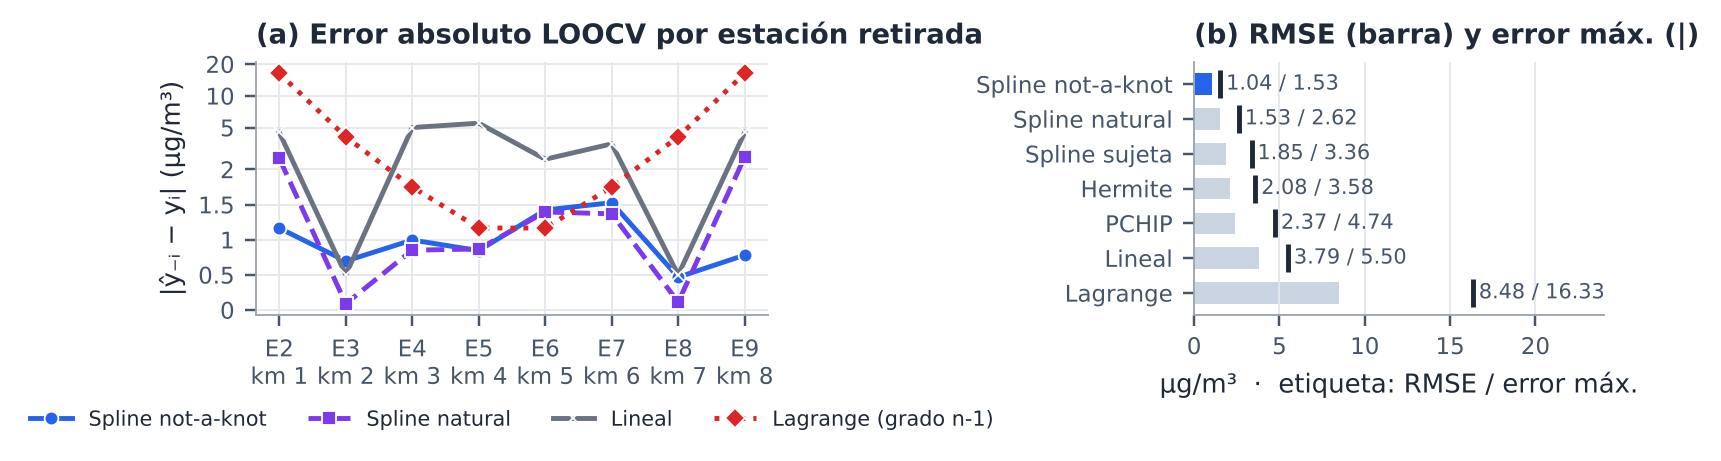
\includegraphics[width=0.92\textwidth]{figuras/fig1_loocv.png}
\caption{Validación LOOCV en los 8 nodos internos. (a) Error absoluto por estación retirada (eje
simétrico-logarítmico). (b) RMSE (barra; resaltado el modelo elegido) y error máximo (marca) por método.}
\label{fig:loocv}
\end{figure*}
El interpolante de Lagrange de grado 9 cumple
$f(x)-P_9(x)=\frac{f^{(10)}(\xi)}{10!}\,\omega(x)$, con $\omega(x)=\prod_{i=0}^{9}(x-x_i)$. Con nodos
equidistantes $|\omega|$ es \RAZONnodal{} veces mayor en el tramo $[0,1]$ que en $[4,5]$: el error se
concentra en los bordes del corredor~\cite{runge1901,trefethen2019}. Además, si las lecturas tienen un error
$|\delta_j|\le\delta$, el error inducido está acotado por $\Lambda\,\delta$, donde
$\Lambda=\max_x\sum_j|\ell_j(x)|$ es la constante de Lebesgue y $\ell_j$ las funciones cardinales. Para
nodos equidistantes $\Lambda_n\sim 2^{n+1}/(e\,n\ln n)$~\cite{trefethen2019}. Medida en los 10 nodos del
corredor (Fig.~\ref{fig:runge}a): $\Lambda=\LEBlag$ para Lagrange (cerca de km 0.32 y \LEBlagkm) frente a
\LEBnak{} (\nak) y \LEBnat{} (natural). Con 30 nodos, Lagrange llega a $\LEBlagTreinta$ mientras el spline
sigue en \LEBnakTreinta{} (Fig.~\ref{fig:runge}b).

\subsection{Mecanismos del spline}
\begin{enumerate}
\item \emph{Grado fijo:} polinomios cúbicos por tramos; el grado no crece con el número de estaciones.
\item \emph{Localidad:} la influencia de una estación decae $\approx 2-\sqrt3\approx0.268$ por tramo. Para
E5 se mide \LOCuno, \LOCdos{} y \LOCtres{} a 1, 2 y 3\,km, mientras que su función cardinal de Lagrange
alcanza \LOClagBorde{} en los tramos extremos: una perturbación en km~4 se amplifica en km 0--1.
\item \emph{Mínima curvatura:} entre las funciones $C^2$ que interpolan los datos, el spline natural
minimiza $\int (f'')^2dx$~\cite{holladay1957,deboor2001}; no puede ``inventar'' oscilaciones. Lagrange
presenta \EXTlag{} extremos locales (los datos tienen 1) y un exceso de variación total de
\VTlag\,\ugm; el \nak, \VTnak\,\ugm{} (un mínimo de \MINnak{} junto a km 9, despreciable).
\item \emph{Convergencia:} con pendientes exactas $\|f-S\|_\infty\le\frac{5}{384}h^4\|f^{(4)}\|_\infty$
~\cite{hall1976}. Sobre una pluma gaussiana de referencia el orden observado es \ORDnak{} (\nak) y
\ORDsujex{} (sujeta exacta), frente a \ORDnat{} (natural) y \ORDlin{} (lineal), Fig.~\ref{fig:conv}a. Para
$1/(1+25x^2)$ el error de Lagrange crece de \RUNGElagIni{} a \RUNGElagFin{} entre 5 y \RUNGEnodosFin{} nodos,
y el del spline baja a \RUNGEsplFin{} (Fig.~\ref{fig:conv}b).
\end{enumerate}

% -------------------------------------------------------------------------------------
\section{Verificación de la implementación}
Se programó el spline con las tres fronteras (sistema de la Sec.~\ref{sec:formulacion} y algoritmo de Thomas) y se comparó con
\texttt{scipy.interpolate.CubicSpline}~\cite{virtanen2020} en la malla uniforme y en las 8 mallas no
uniformes de la LOOCV: la diferencia máxima de coeficientes es $\VERmax$ y todos los sistemas resultaron
estrictamente diagonal dominantes. Los saltos de $S$, $S'$ y $S''$ en los nodos internos son
$\le\CONTmax$ (clase $C^2$) y, en el \nak, el salto de $S'''$ en $x_1$ y $x_8$ es nulo, como exige la
condición. Estas comprobaciones forman parte de 26 pruebas automáticas (\texttt{pytest}).

% -------------------------------------------------------------------------------------
\section{Validación cruzada leave-one-out}
\begin{figure*}[!t]
\centering
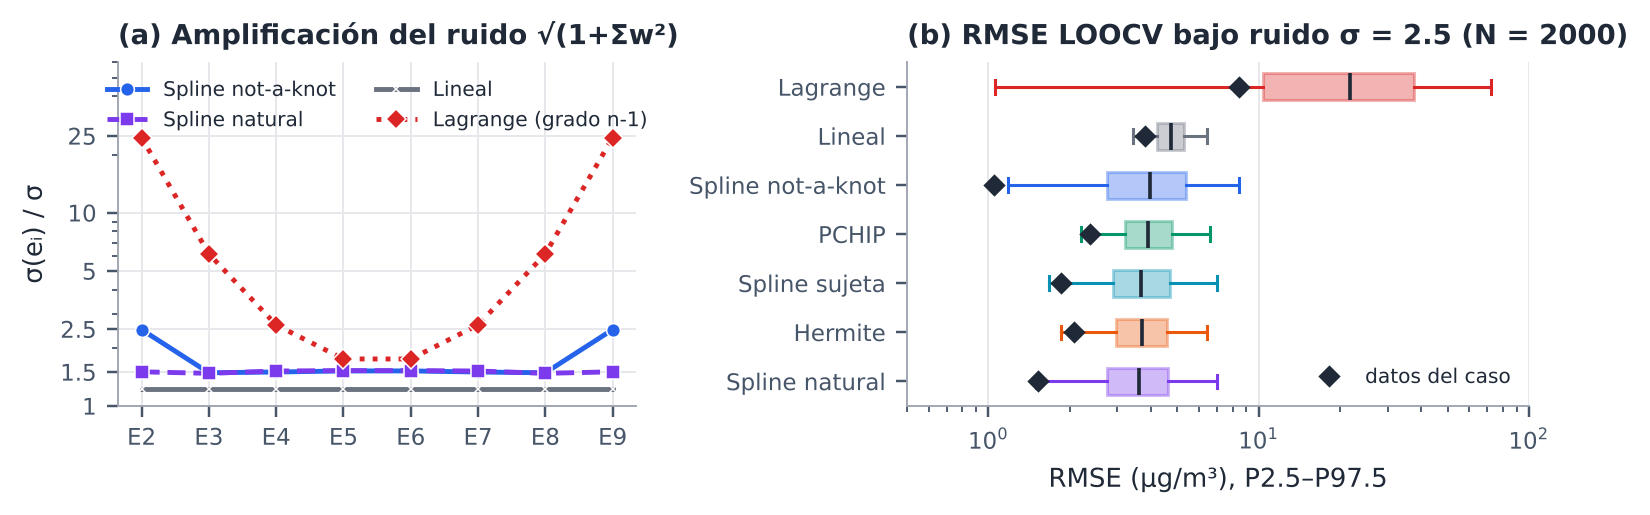
\includegraphics[width=0.92\textwidth]{figuras/fig4_robustez_ruido.png}
\caption{Robustez. (a) Factor de amplificación del ruido en el error LOOCV de cada estación. (b) Distribución
del RMSE LOOCV bajo ruido (caja: P25--P75; bigotes: P2.5--P97.5) y RMSE con los datos del caso (rombo).}
\label{fig:ruido}
\end{figure*}
\subsection{Esquema}
Para cada estación interna $E_{i+1}$, $i=1,\dots,8$, se retira el dato, se ajusta el modelo con las 9
restantes (malla no uniforme con un hueco de 2\,km) y se predice el valor retirado:
\begin{equation}
e_i=\hat y_{-i}(x_i)-y_i,\quad \text{RMSE}=\sqrt{\tfrac18\textstyle\sum e_i^2},\quad
e_{\max}=\max_i|e_i| .
\end{equation}
E1 y E10 no se retiran porque su predicción sería una extrapolación. La LOOCV simula exactamente la falla
de una estación~\cite{hastie2009} y, al predecir a través de un hueco de $2h$, es una estimación
conservadora del error del modelo final con $h=1$\,km (Código~\ref{lst:loocv}).

\begin{lstlisting}[float=!t, caption={Esquema LOOCV (extracto de \texttt{modelado\_validacion.py}).}, label=lst:loocv]
def loocv(x, y, nombres):
    filas = []
    for i in range(1, len(x) - 1):      # nodos internos
        m = np.ones(len(x), bool)
        m[i] = False                    # retirar la estación
        mods = construir_modelos(x[m], y[m])   # 9 datos
        filas.append({n: float(mods[n](x[i])) - y[i]
                      for n in nombres})  # e_i con signo
    e = pd.DataFrame(filas)
    return np.sqrt((e**2).mean()), e.abs().max()   # RMSE, e_max
\end{lstlisting}

\begin{table}[!t]
\caption{LOOCV: error con signo $e_i$ por estación retirada y métricas (\ugm). En negrita, el mejor.}
\label{tab:loocv}
\centering\scriptsize
\setlength{\tabcolsep}{2.2pt}
\begin{tabular}{@{}l r *{7}{r}@{}}
\toprule
Est. & $y_i$ & NaK & Nat. & Suj. & Herm. & PCHIP & Lin. & Lagr. \\
\midrule
E2 & 52 & $-1.16$ & $+2.55$ & $+3.32$ & $+3.58$ & $+2.95$ & $+4.50$ & $+16.33$ \\
E3 & 68 & $+0.70$ & $+0.09$ & $-0.14$ & $+0.50$ & $+0.50$ & $+0.50$ & $-4.08$ \\
E4 & 85 & $-1.00$ & $-0.85$ & $-0.79$ & $-1.67$ & $-1.52$ & $-5.00$ & $+1.75$ \\
E5 & 92 & $-0.84$ & $-0.87$ & $-0.88$ & $-1.17$ & $-4.74$ & $-5.50$ & $-1.17$ \\
E6 & 88 & $+1.42$ & $+1.39$ & $+1.38$ & $+1.33$ & $-0.08$ & $-2.50$ & $+1.17$ \\
E7 & 79 & $-1.53$ & $-1.37$ & $-1.30$ & $-1.67$ & $-1.49$ & $-3.50$ & $-1.75$ \\
E8 & 63 & $+0.47$ & $-0.11$ & $-0.33$ & $+0.00$ & $-0.20$ & $+0.50$ & $+4.08$ \\
E9 & 48 & $-0.78$ & $+2.62$ & $+3.36$ & $+3.58$ & $+2.96$ & $+4.50$ & $-16.33$ \\
\midrule
\multicolumn{2}{@{}l}{RMSE} & \textbf{1.04} & 1.53 & 1.85 & 2.08 & 2.37 & 3.79 & 8.48 \\
\multicolumn{2}{@{}l}{MAE} & \textbf{0.99} & 1.23 & 1.44 & 1.69 & 1.81 & 3.31 & 5.83 \\
\multicolumn{2}{@{}l}{$e_{\max}$} & \textbf{1.53} & 2.62 & 3.36 & 3.58 & 4.74 & 5.50 & 16.33 \\
\multicolumn{2}{@{}l}{Peor} & E7 & E9 & E9 & E2 & E5 & E5 & E2 \\
\bottomrule
\end{tabular}

\end{table}

\subsection{Resultados}
La Tabla~\ref{tab:loocv} y la Fig.~\ref{fig:loocv} muestran que el spline \nak{} es el mejor en las tres
métricas: RMSE\,=\,\RMSEnak, MAE\,=\,\MAEnak{} y $e_{\max}$\,=\,\EMAXnak\,\ugm{} (\PEORnak, flanco de
descenso). Las fronteras natural y sujeta fallan en E2 y E9, justo donde actúa su hipótesis de borde.
Lagrange (grado 8 sobre nodos no equidistantes) comete errores de $\pm$\EMAXlag\,\ugm{} en E2/E9, y la lineal
subestima el pico de E5 en 5.5\,\ugm: su alerta roja queda en km \ROlinDesde--\ROlinHasta{} frente a
\ROdesde--\ROhasta{} del spline (\DESFASElin\,m de diferencia).

% -------------------------------------------------------------------------------------
\section{Robustez de la validación ante el ruido}
\subsection{Amplificación analítica}
Para los métodos lineales en los datos (todos salvo PCHIP) el vector de errores LOOCV es $e=My$, con $M$ de
$8\times10$. Si cada lectura tiene ruido independiente $N(0,\sigma^2)$, la desviación de $e_i$ es
$\sigma\|M_i\|_2=\sigma\sqrt{1+\sum_jw_{ij}^2}$. Para la lineal es $\sqrt{1.5}=\FAClin$ en todas las
estaciones; para el \nak{} es $\approx1.5$ en el interior pero \FACnakBorde{} en E2/E9; la natural,
\FACnatBorde; Lagrange, \FAClagBorde{} (Fig.~\ref{fig:ruido}a).

\subsection{\texorpdfstring{LOOCV bajo ruido $\sigma=2.5$\,\ugm}{LOOCV bajo ruido sigma = 2.5}}
Se repitió la LOOCV en \NMC{} realizaciones $y+\varepsilon$ (semilla \SEMILLA;
Fig.~\ref{fig:ruido}b). Con ruido fuerte, los métodos cúbicos $C^1$/$C^2$ quedan estadísticamente empatados
(medias de \MCnat{} a \MCnak\,\ugm{} con intervalos muy superpuestos) y ninguno domina: el \nak{} obtiene el
menor RMSE en el \MCganaNak\,\% de las realizaciones, pero su mayor sensibilidad en los bordes eleva su media. Lineal (\MClin) y Lagrange
(\MClag) siguen siendo peores. Coincide con la banda de la §8 del cuaderno (replicada aquí): ancho máximo
\BANDAmax\,\ugm{} en km \BANDAmaxkm{} y mínimo \BANDAmin{} en km \BANDAminkm.

\subsection{Interpretación}
El RMSE observado del \nak{} (\RMSEnak) cae en el percentil \PCTnak{} de su distribución bajo ruido: si
cada lectura tuviera ruido independiente de 2.5\,\ugm{} sería muy improbable un error tan bajo. Atribuyendo
toda la discrepancia LOOCV a ruido, éste sería a lo sumo $\approx$\SIGef\,\ugm{}; las lecturas del caso se
comportan como promedios. Por tanto, $\sigma=2.5$ es un escenario \emph{conservador}, adecuado para alertas
sanitarias. Por último, los tramos de alerta (amarilla km \AMdesde--\AMhasta; roja km \ROdesde--\ROhasta)
cambian a lo sumo \DESFASEsplines\,m entre las fronteras \nak, natural y sujeta, y \DESFASEherPch\,m con
Hermite o PCHIP: con una malla de 100\,m, la elección de frontera no altera ninguna alerta.

% -------------------------------------------------------------------------------------
\section{Conclusiones y entregables al equipo}
\begin{itemize}
\item \textbf{Modelo:} spline cúbico \nak{} (\texttt{CubicSpline}, \texttt{bc\_type="not-a-knot"}), clase
$C^2$, orden $O(h^4)$, seleccionado por LOOCV y sin hipótesis artificiales de borde.
\item \textbf{KPIs para Integración y Estrategia:} RMSE\,=\,\RMSEnak\,\ugm, $e_{\max}$\,=\,\EMAXnak\,\ugm,
$-$\REDlin\,\% de RMSE frente a la lineal y $-$\REDlag\,\% frente a Lagrange.
\item \textbf{Para Algoritmos y Simulación:} la incertidumbre es mayor en km 0--1 y 8--9 (factor
\FACnakBorde); la banda Monte Carlo debe acompañar siempre a la alerta.
\item \textbf{Hallazgo de validación:} la búsqueda de tramos de alerta para lineal y Lagrange perdía las
raíces que caen sobre la malla (km 4.5 con umbral 90); quedó corregida y con prueba de regresión.
\item \textbf{Limitaciones y trabajo futuro:} modelo 1-D, 10 datos y 8 pliegues; no modela viento ni
tráfico. Con ruido real del orden de $\sigma=2.5$ convendría un spline de \emph{suavizado} o kriging.
\end{itemize}

% -------------------------------------------------------------------------------------
\begin{thebibliography}{9}
\bibitem{burden2017} R. L. Burden, J. D. Faires y A. M. Burden, \emph{Análisis numérico}, 10.ª ed.
Cengage Learning, 2017.
\bibitem{deboor2001} C. de Boor, \emph{A Practical Guide to Splines}, ed. rev.
Springer, 2001.
\bibitem{hall1976} C. A. Hall y W. W. Meyer, ``Optimal error bounds for cubic spline interpolation,''
\emph{J. Approx. Theory}, vol.~16, no.~2, pp.~105--122, 1976.
\bibitem{trefethen2019} L. N. Trefethen, \emph{Approximation Theory and Approximation Practice}, ed.
ampliada. SIAM, 2019.
\bibitem{runge1901} C. Runge, ``Über empirische Funktionen und die Interpolation zwischen äquidistanten
Ordinaten,'' \emph{Z. Math. Phys.}, vol.~46, pp.~224--243, 1901.
\bibitem{holladay1957} J. C. Holladay, ``A smoothest curve approximation,'' \emph{Math. Tables Aids
Comput.}, vol.~11, no.~60, pp.~233--243, 1957.
\bibitem{hastie2009} T. Hastie, R. Tibshirani y J. Friedman, \emph{The Elements of Statistical Learning},
2.ª ed. Springer, 2009.
\bibitem{virtanen2020} P. Virtanen \emph{et al.}, ``SciPy 1.0: Fundamental algorithms for scientific
computing in Python,'' \emph{Nat. Methods}, vol.~17, pp.~261--272, 2020.
\end{thebibliography}

\end{document}
